\chapter{Аналитический раздел}
\label{cha:analysis}
%
% % В начале раздела  можно напомнить его цель
%

В данном разделе будут рассмотрены перспективы работы с микроконтроллерами семейства STM32 и существующие решения поставленной задачи, 
будут проанализированы методы моделирования трёхмерных объектов, из которых будет выбран метод решения поставленной задачи.

\section{Описание платформы STM32}

Производитель микроконтроллеров семейства STM32, компания STMicroelectronics, является одним из мировых лидеров по производству и продажам микроконтроллеров и прочно закрепилась на российском рынке микроэлектроники. 32-битные микроконтроллеры от этого производителя нашли широкий спектр приложений, разрабатываемых средними и малыми клиентами (так называемый массовый рынок) в рамках промышленных применений \cite{STMicroelectronics_description}.

Одной из главных причин популярности микроконтроллеров семейства STM32 является наличие обширной экосистемы, которая развивается с течением времени. К микроконтроллерам семейства STM32 можно подключать всё больше периферийных устройств для решения различных задач. Также экосистема STM32 имеет программную поддержку в виде бесплатной среды разработки и интегрируется с программными инструментами сторонних компаний, что даёт большую гибкость при разработке программных продуктов для STM32.

Стоит отметить, что рассматриваемое семейство микроконтроллеров имеет ряд аналогов, в том числе и от российских производителей, благодаря чему имеется возможность в будущем перенести разработки с STM32 на отечественную аппаратную платформу.

\section{Оценка существующих инструментов}

Поиск по популярному сервису для хостинга IT проектов GitHub \cite{git0} показал, что уже существуют четыре программных инструмента с открытым исходным кодом, решающих поставленную задачу. Их оценку можно проводить по следующим критериям:
\begin{enumerate}
	\item[1)] производительность;
	\item[2)] универсальность;
	\item[3)] качество пользовательского интерфейса.
\end{enumerate}

Рассмотрим существующие программные решения.

\subsection{Библиотека для построения трёхмерных поверхностных моделей}
Библиотека, представленная в \cite{git1}, предоставляет функционал для построения трёхмерных моделей и рассчитан на конкретные дисплеи. 
Визуализация осуществляется с помощью алгоритма построчного сканирования, использующего Z-буфер и простую модель освещения с учётом 
плоского затенения. Важно заметить, что в коде библиотеки не используются низкоуровневые оптимизации. Исходные данные для работы 
алгоритмов задаются в коде программы, то есть отсутствует возможность загрузки модели из файла или с помощью графического 
пользовательского интерфейса.

\subsection{Библиотека для создания анимаций на основе векторной трёхмерной графики}
Библиотека, представленная в \cite{git2}, предназначена для рендеринга трёхмерных анимаций с частотой кадров до 80 кадров в секунду. Однако этот инструмент предназначен 
для работы с конкретными моделями микроконтроллера и дисплея, обладающего относительно низким разрешением — 128x160 пикселей. Как и в 
предыдущем случае, исходные данные задаются в коде программы.

\subsection{Библиотека для создания анимаций трёхмерных каркасных моделей}
Функционал библиотеки, представленной в \cite{git3}, позволяет осуществлять рендеринг трёхмерных анимаций на конкретной модели дисплея с использованием низкоуровневых 
оптимизаций. Но стоит отметить, что при изображении трёхмерной модели не используются алгоритмы удаления невидимых линий и поверхностей, 
что очень сильно упрощает данный инструмент. Как и в предыдущих примерах, исходные данные задаются в коде программы.

\subsection{Частичная реализация библиотеки OpenGL для STM32}
Программный инструмент, представленный в \cite{git4}, рассчитан на конкретные модели микроконтроллеров и реализует базовый функционал популярной графической библиотеки 
OpenGL, а именно построение трёхмерных моделей с помощью алгоритма удаления невидимых линий и поверхностей, использующего Z-буфер. В 
алгоритмах не учитывается модель освещения, тени, текстурирование и сглаживание. Несмотря на сложность используемых алгоритмов, инструмент 
обладает высоким быстродействием за счёт наличия низкоуровневых оптимизаций. Данная библиотека, как и предыдущие, не предусматривает 
взаимодействия с пользователем и строит трёхмерные модели, заданные в коде программы.

После анализа библиотек можно выделить недостатки, встречающиеся у существующих программных инструментов:
\begin{enumerate}
	\item[1)] ориентированность исключительно на конкретные модели микроконтроллеров и дисплеев;
	\item[2)] относительно низкая производительность за счёт отсутствия низкоуровневых оптимизаций;
	\item[3)] способ задания исходных данных затрудняет использование графического инструмента;
	\item[4)] отсутствует пользовательский интерфейс;
	\item[5)] отсутствует масштабируемость.
\end{enumerate}

Обладая перечисленными выше недостатками, программный инструмент не может использоваться в полномасштабных проектах.

Также стоит отметить, что популярные графические библиотеки, такие как OpenGL \cite{opengl}, Direct3D \cite{direct3d} или Vulkan \cite{vulkan}, которые повсеместно используются при решении задач компьютерной графики на различных аппаратных платформах, не поддерживают работу с микроконтроллерами семейства STM32.

Отсюда следует необходимость разработки программного инструмента, который решал бы поставленную задачу для платформы STM32, не имея при этом недостатков, присущих рассмотренным ранее альтернативам.

\section{Требования к алгоритмам визуализации трёхмерных объектов}
При выборе алгоритма удаления невидимых линий и поверхностей необходимо учитывать особенности решаемой задачи:
\begin{enumerate}
	\item[1)] микроконтроллеры имеют относительно небольшую вычислительную мощность;
	\item[2)] объём доступной памяти микроконтроллеров очень ограничен и составляет, как правило, не более 0.5–2 Мб.
\end{enumerate}

Исходя из этих особенностей, можно сформулировать требования к алгоритмам:
\begin{enumerate}
	\item[1)] компактность – алгоритмы должны задействовать минимальное количество памяти, используя структуры данных, не содержащие избыточной информации;
	\item[2)] простота и лаконичность – алгоритмы должны быть простыми, чтобы итоговый исполняемый файл занимал как можно меньше места в памяти микроконтроллера;
	\item[3)] быстродействие – микроконтроллер, не обладающий большими вычислительными мощностями, должен выполнять алгоритмы за приемлемое время.
\end{enumerate}
% - короткое тире, – длинное

Ввиду того, что в данном случае ограничение по памяти сильнее ограничения по времени, эффективность алгоритмов по памяти будет самым важным критерием оценки алгоритмов.

Рассмотрим основные алгоритмы построения трехмерной сцены \cite{Rogers}.

\section{Анализ алгоритмов удаления невидимых линий и поверхностей}
\subsection{Алгоритм Робертса}
Алгоритм Робертса – метод удаления невидимых линий и поверхностей, работающий в объектном пространстве. Основные этапы работы алгоритма Робертса:
\begin{enumerate}
	\item[0)] подготовка исходных данных: разбиение невыпуклых тел на выпуклые, составление корректной матрицы каждого тела;
	\item[] Далее для каждого тела сцены:
	\item[1)] удаление рёбер, экранируемых самим телом;
	\item[2)] удаление рёбер, экранируемых другими телами (если на сцене находятся несколько тел);
	\item[3)] удаление линий пересечения тел, экранируемых самими телами и другими телами, связанными отношением протыкания.
\end{enumerate}

Математические методы, используемые в этих этапах, дают очень высокую точность вычислений за счёт того, что алгоритм Робертса работает в объектном пространстве. 

В то же время, каждый этап алгоритма основан на трудоёмких математических вычислениях, сложность которых растёт как квадрат числа объектов сцены. Стоит отметить, что алгоритм Робертса можно оптимизировать, однако реализовать эти оптимизации крайне сложно.

\subsection{Алгоритм Варнока}
Алгоритм Варнока решает задачу удаления невидимых линий и поверхностей в пространстве изображения. Его идея состоит в том, что на обработку областей изображения, содержащих мало информации, должно тратиться очень мало времени, и наоборот. 

В пространстве изображения рассматривается окно и решается вопрос о том, достаточно ли оно простое для визуализации. Если это не так, то окно разбивается на подокна до тех пор, пока условие не будет выполняться. 

В конкретных реализациях могут использоваться различные методы разбиения окна и рассматриваться различные случаи взаимного расположения многоугольников относительно окна. Усложнение критериев и способов разбиения способно значительно повысить эффективность алгоритма. 

\begin{figure}[h]
	\centering
	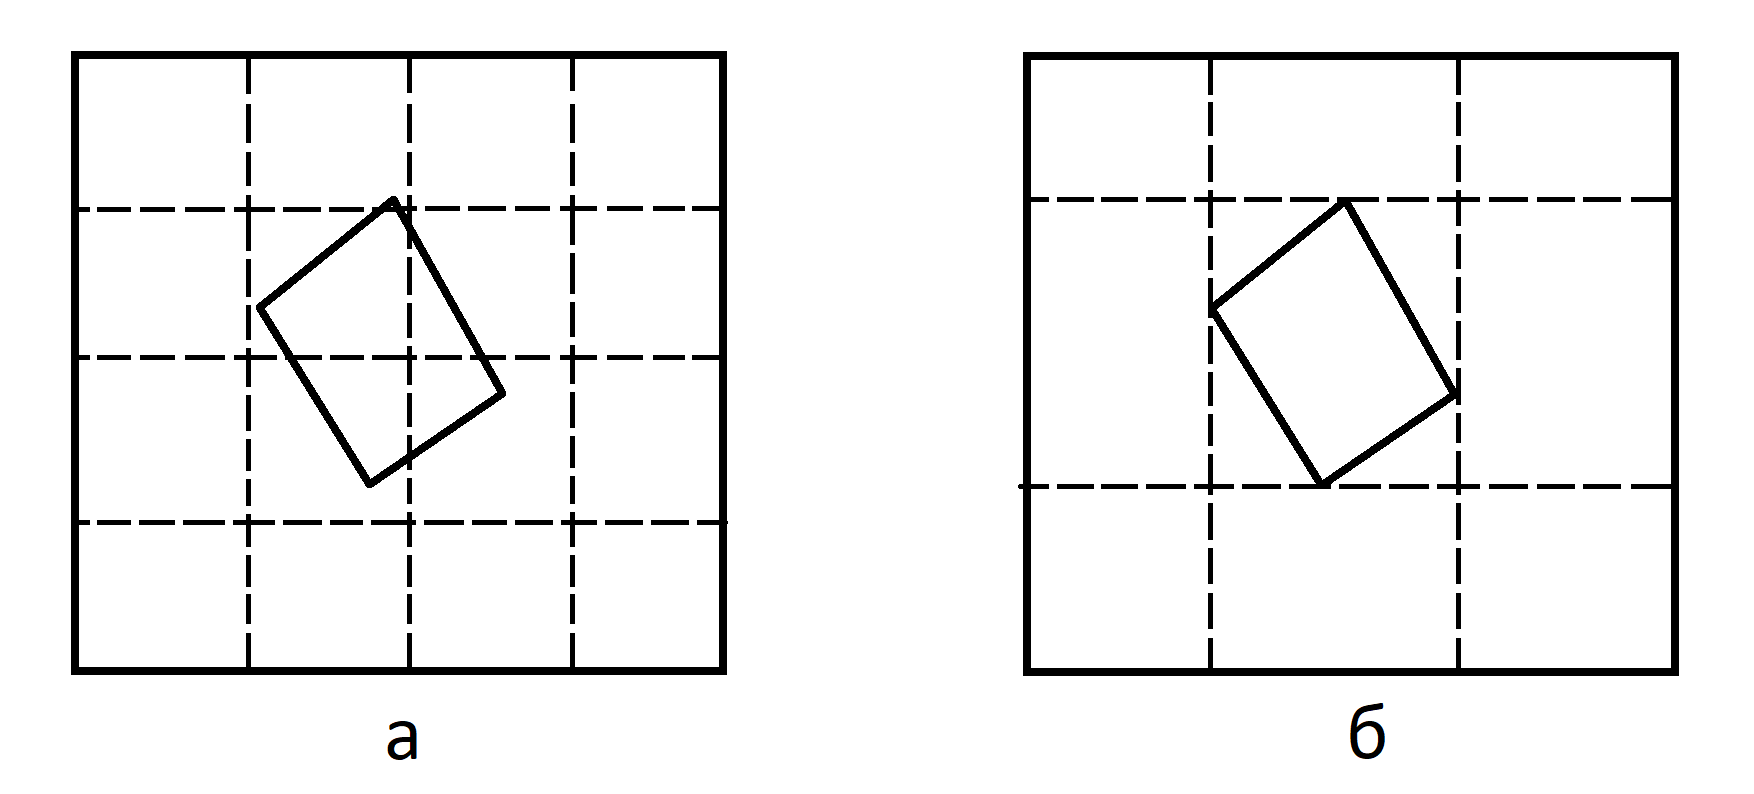
\includegraphics[width=\textwidth ]{img/subdivide.png}
	\caption{Сравнение двух способов разбиения окна}
\end{figure} 

Также в целях оптимизации можно выполнять предварительную сортировку многоугольников по глубине с целью оптимизации поиска многоугольников, охватывающих рассматриваемое окно.

Стоит отметить, что рекурсивное разбиение окна, в зависимости от числа пересечений объектов, может стать как положительной, так и отрицательной стороной алгоритма Варнока. Чем меньше пересечений объектов сцены, тем быстрее выполнится алгоритм.

\subsection{Алгоритм Вейлера-Азертона}
В алгоритме Вейлера-Азертона  производится попытка минимизировать количество шагов в алгоритме Варнока путем разбиения окна вдоль границ многоугольника.

Алгоритм решения задачи удаления невидимых линий и поверхностей удаления целиком базируется на алгоритме отсечения тех же авторов. Работа будет вестись с проекциями многоугольников, то есть в пространстве изображения. Алгоритм отсечения позволяет найти как внутренние, так и внешние отсечения, что важно.

Основные этапы алгоритма Вейлера-Азертона:
\begin{enumerate}
	\item[1)] сортировка многоугольников по глубине;
	\item[2)] отсечение всех многоугольников сцены по границе ближайшего к наблюдателю многоугольника;
	\item[3)] удаление многоугольников, экранируемых ближайшим к наблюдателю многоугольником;
	\item[4)] рекурсивное разбиение многоугольников, выполняемое в том случае, когда многоугольники, расположенные в списке за ближайшим многоугольником.
\end{enumerate}

К недостаткам алгоритма можно отнести то, что он не справляется с ситуацией пересечения двух многоугольников, поэтому в нём приходится отдельно рассматривать этот случай и разбивать один из них по линии пересечения многоугольников.

Ввиду больших затрат времени и памяти на выполнение алгоритма отсечения Вейлера-Азертона, основанного на работе с двунаправленными циклическими списками, соответствующий алгоритм удаления невидимых линий и поверхностей нельзя считать более эффективным, чем алгоритм Варнока.

\subsection{Алгоритм, использующий Z-буфер}
Алгоритм, использующий Z-буфер является одним из простейших алгоритмов удаления невидимых поверхностей, который работает в пространстве изображения.

Для своей работы он использует два буфера: буфер кадра, хранящий цвет (интенсивность) каждого пикселя в пространстве изображения, и Z-буфер (буфер глубины), хранящий информацию о координате Z для каждого пикселя. Вначале в Z-буфер заносятся минимальные значения Z, а буфер кадра заполняется фоновыми значениями. Затем каждый многоугольник преобразуется в растровую форму и записывается в буфер кадра, при этом не производится начального упорядочения.

В процессе работы глубина (значение координаты Z) каждого нового пикселя, который надо занести в буфер кадра, сравнивается с глубиной того пикселя, который уже занесён в Z -буфер. Если это сравнение показывает, что новый пиксель расположен ближе к наблюдателю, чем пиксель, уже находящийся в буфере кадра, то новый пиксель заносится в буфер кадра. Кроме того, производится корректировка Z-буфера: в него заносится глубина нового пикселя. Если же глубина рассматриваемого пикселя меньше глубины пикселя, хранящегося в Z-буфере, то никаких действий производить не надо.

Достоинства:
\begin{itemize}
	\item простота визуализации сцен любой сложности;
	\item отсутствие сортировки объектов сцены по глубине, как в других алгоритмах.
\end{itemize}

Недостатки:
\begin{itemize}
	\item большой объём задействуемой памяти;
	\item трудоёмкость устранения лестничного эффекта;
	\item трудоёмкость реализации эффектов, связанных с полупрозрачностью, просвечиванием и рядом других специальных задач, повышающих реалистичность изображения.
\end{itemize}

Последний недостаток связан с тем, что пиксели заносятся в буфер кадра в произвольном порядке. Это затрудняет получение информации, необходимой для методов, основывающихся на предварительном анализе изображения. Проблема относительно легко решается использованием методов постфильтрации.

Ввиду того, что алгоритм требует объём памяти, в разы превышающий тот, который имеют микроконтроллеры семейства STM32, его рассмотрение для реализации поставленной задачи не имеет смысла.

\subsection{Алгоритм построчного сканирования, использующий Z-буфер}
Использование методов построчного сканирования в алгоритме, использующем Z-буфер, решает проблему использования большого количества памяти за счёт того, что буферизуется не весь экран, а только одна сканирующая строка.

Алгоритмы построчного сканирования работают в пространстве изображения и обрабатывают сцену в порядке прохождения сканирующей строки. Для каждого пикселя вычисляется глубина многоугольника, пересекающего рассматриваемую сканирующую строку. 

Количество вычислений можно сократить, если использовать понятие интервалов. Решение задачи удаления невидимых поверхностей сводится к выбору видимых отрезков в каждом интервале, полученном путём деления сканирующей строки проекциями точек пересечения рёбер.

За то, что алгоритм построчного сканирования, использующий Z-буфер, решает проблему большого расхода памяти, приходится расплачиваться дополнительными вычислениями, связанными с использованием списка активных многоугольников.

\subsection{Алгоритм, использующий список приоритетов}
В основе алгоритма лежит сортировка объектов по приоритету, то есть по глубине объектов сцены или их расстоянию от точки наблюдения. Сначала изображаются объекты, расположенные дальше всех от наблюдателя, а затем их перекрывают объекты, находящиеся ближе к наблюдателю.

После сортировки объектов сцены по глубине и получается первоначальный список приоритетов. Далее он корректируется путём выполнения серии тестов на экранирование для каждой пары многоугольников в списке. Эти тесты достаточно трудоёмкие с точки зрения эффективности по времени и сложности реализации.

Также стоит отметить, что в алгоритме очень сложно идентифицируются случаи пересечения и циклического перекрытия многоугольников сцены.

\subsection{Алгоритм определения видимых поверхностей путем трассировки лучей}
В алгоритме, использующем трассировку лучей, отслеживаются (трассируются) лучи, идущие от наблюдателя к объекту. Такая трассировка называется обратной.

Для определения видимых поверхностей от наблюдателя, находящегося в бесконечности на положительном направлении оси Z, испускаются лучи, проходящие через каждый пиксель картинной плоскости. Траектория каждого луча отслеживается, чтобы определить пересечения объектов сцены с данным лучом. Пересечение с максимальным значением z представляет видимую поверхность для данного пикселя картинной плоскости.

\begin{figure}[h]
	\centering
	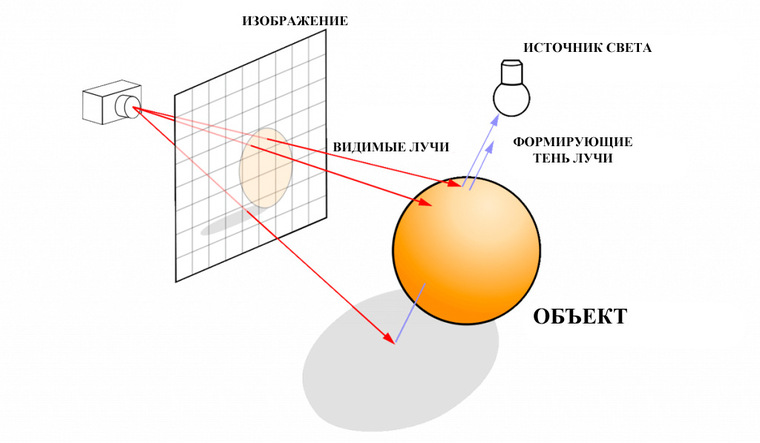
\includegraphics[width=\textwidth ]{img/raytracing.png}
	\caption{Иллюстрация алгоритма определения видимых поверхностей путем трассировки лучей}
\end{figure} 

Поиск пересечений является наиболее важным и трудоемким элементом этого алгоритма, поэтому его быстродействие существенно зависит от скорости их определения. Однако, несмотря на трудоёмкость этой процедуры, вычислительная сложность метода линейно зависит от количества объектов сцены. 

Главное преимущество алгоритма трассировки лучей – качество и реалистичность изображения. Также при использовании данного алгоритма нетрудно реализовать наложение света и тени на объекты.

К недостаткам данного алгоритма можно отнести производительность, так как трассировка большого количества лучей является очень трудоёмким процессом. Учёт прозрачности, усложняющий процесс трассировки лучей, только усугубит проблему.

\section{Анализ алгоритмов закрашивания}
\subsection{Простая закраска}
При использовании простой закраски вся грань многогранника закрашивается одним уровнем интенсивности, который вычисляется по закону Ламберта.

Предпосылки к использованию простой закраски:
\begin{enumerate}
	\item[1)] источник света находится на бесконечном удалении от объектов сцены;
	\item[2)] наблюдатель находится на бесконечном удалении от объектов сцены;
	\item[3)] закрашиваемая грань реально существует, а не является результатом аппроксимации другой поверхности.
\end{enumerate}

Из последнего пункта вытекает недостаток алгоритма простой закраски: он не подходит для закраски криволинейных поверхностей. Также к недостаткам алгоритма можно отнести то, что он никак не учитывает отражённый свет.

Главное преимущество алгоритма - простота реализации. Если поместить наблюдателя в бесконечность, то данный алгоритм хорошо подойдёт для решения поставленной задачи.

\subsection{Закраска по Гуро}
Закраска по Гуро предполагает билинейную интерполяцию интенсивностей. В результате вычисления интенсивности в каждой точке грани создаётся иллюзия гладкой криволинейной поверхности.

Закраска по Гуро хорошо сочетается с простой моделью освещения с диффузным отражением.

Несмотря на то, что применение закраски по Гуро сильно улучшает качество изображения, этот алгоритм имеет свои недостатки:
\begin{enumerate}
	\item[1)] появляется эффект полос Маха;
	\item[2)] в результате сглаживания теряется граница между гранями многогранника, что в некоторых случаях может дать неверный результат.
\end{enumerate}

Последний недостаток можно устранить, разбивая грани многогранника или создавая возмущения в уравнения нормалей к граням, чтобы сделать их разными. Однако такой подход увеличит объём вычислений.

\subsection{Закраска по Фонгу}
Закраска по Фонгу предполагает билинейную интерполяцию нормалей к граням многогранника. Такой подход требует больших вычислительных затрат, чем закраска по Гуро, и в результате даёт более качественное изображение, устраняя большинство недостатков предыдущего алгоритма.

\begin{figure}[h]
	\centering
	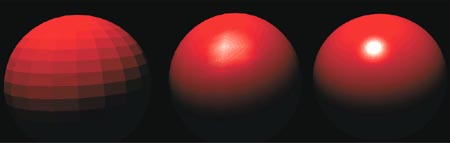
\includegraphics[width=\textwidth ]{img/shading.png}
	\caption{Сравнение методов закраски: слева – простая, в центре – Гуро, справа – Фонга}
\end{figure}

К недостаткам закраски по Гуро и по Фонгу можно отнести ошибки при закраске невыпуклых многоугольников, а также большую вычислительную сложность и ресурсоёмкость.

\section{Вывод из аналитического раздела}
В данном разделе были проанализированы перспективы работы с семейством STM32, существующие решения поставленной задачи, а также методы моделирования трёхмерных объектов. Ввиду отсутствия универсальных программных инструментов для платформы STM32, которые могли бы решать задачи трёхмерной компьютерной графики, а также с учётом переносимости программного обеспечения на отечественные платформы, разработка имеет актуальность.

Несмотря на перспективы импортозамещения, для разработки была выбрана оригинальная платформа STM32 ввиду её более развитой экосистемы и наличия большого количества материалов по работе с микроконтроллерами этого семейства. Это упростит работу с микроконтроллером и его периферийными устройствами, а также разработку программных продуктов для данной платформы, что позволит уделить больше внимания задачам компьютерной графики.

В качестве алгоритма удаления невидимых линий и поверхностей был выбран алгоритм Варнока ввиду его компактности и относительно небольшой вычислительной сложности, а в качестве алгоритма закраски -  простая закраска по причине её относительно небольшой ресурсоёмкости и вычислительной сложности.




%%% Local Variables:
%%% mode: latex
%%% TeX-master: "rpz"
%%% End:
